\section{ Implementation and Used Technologies}
\phantomsection

For a better understanding of the application, on how it works, how it behaves for the patient and in general for those who will use it, it is better and I would say important to describe the technologies that were used to build Kyno. In this chapter will be analysed the implementation of the features that presents the Kyno as a software, will be shown some code samples and analysed the solutions that were choosed to develop the application.

\subsection{System Requirements}
In order to run the application and to have a nice user experience, there is needed for the client to have 2 componenets.

\begin{itemize}
\item A computer, laptop or any system/device where you can install a desktop application

\item A Leap Motion tracking device with again the ability to install software on your device.
\end{itemize}

As we can see the requirements are not that simple and easy to get since the Leap Motion can be bought only online from USA and cost almost 100 euros. However the application will come with the Leap Motion controller in the set.

\subsection {Technologies Used}
\subsubsection {Unity}
Unity is a powerful cross-platform 3D engine and a user friendly development environment. Easy enough for the beginner and powerful enough for the expert.
\\
\textbf{Why Unity over others?}

The main "pro" of Unty is that it's crazy fast. I'm not talking about performance here, but about development speed. It has:

\begin{itemize}
\item \textbf{Unified asset pipeline}. No need to spend time on resource subsystem at all, no buggy import routines to write and fix: just drop a file into folder, and it works.
\item \textbf{Integrated level editor}. No need to spend time on level tools: just get straight to business.

\item \textbf{Great tweaking and debugging support}.All your scripting variables are shown in the editor right as you play, and can be changed on the fly too - and all this without writing a single line of code. Pause the application anytime, or step through code one statement at a time.

\item \textbf{Quite comprehesive library of ready-made components}. Rendering, sound, physics, controls - a lot of "boilerplate" code is already written so that you can focus on the application and not on how to create an engine.
\end{itemize}

One aspect is that Unity is a game engine and editor that publishes almost anywhere. What does it mean “everywhere”? One can divide the game world in four continents: consoles, smartphones, desktop (installed), browser.  Unity runs in most “countries” from all these continents – as shown in \mbox{figure \ref{everywhere}}.
\begin{figure}[!h]
\centering
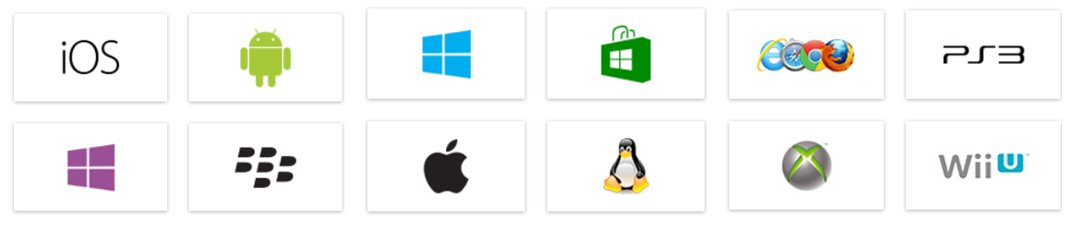
\includegraphics[ width = 14cm]{everywhere}
\caption{Exercising state diagram \cite{multiplatform}}\label{everywhere}
\end{figure}

Application created in Unity can be deployed into multiple platforms simply by downloading and installing support of these platform. After that offcourse by changing your code so that it will work on other platform too.

So let's see 2 examples in of how Unity handles a mouse input in a desktop application and fingers input in a mobile application.
\begin{lstlisting}[caption={Mouse input for desktop application in Unity \cite{mousedown}.},label={mouseInput}]
 void Update() {
         if (Input.GetMouseButtonDown(0))
             Debug.Log("Pressed left click.");
         
         if (Input.GetMouseButtonDown(1))
             Debug.Log("Pressed right click.");
         
         if (Input.GetMouseButtonDown(2))
             Debug.Log("Pressed middle click.");
         
     }
\end{lstlisting}

As we can see \autoref{mouseInput}  returns true during the frame the user pressed the given mouse button. Either will be left click, middle or right click.

\begin{lstlisting}[caption={Multiple touch input for mobile application in Unity \cite{multipletouch}.},label={touchInput}]
void Update () 
    {
        Touch myTouch = Input.GetTouch(0);
        Touch[] myTouches = Input.touches;
        for(int i = 0; i < Input.touchCount; i++)
        {
            //Do something with the touches
        }
    }
\end{lstlisting}

In \autoref{touchInput} Unity handles multi-touch by giving you the number of touches on the screen during a given frame, and/or gives you an array of all touches during a frame. While myTouch will be the first touch the user did and myTouches will be the total amount of touches the user does.

This way Unity does for every platform, it is a console, it is a desktop computer, a mobile phone or web browser. Unity make life easire.
\subsubsection {Leap Motion}

The Leap Motion controller is a small USB peripheral device which is designed to be placed on a physical desktop, facing upward. It can also be mounted onto a virtual reality headset. Using two monochromatic IR cameras and three infrared LEDs, the device observes a roughly hemispherical area , to a distance of about 80 cm \mbox{figure \ref{area}}. This range is limited by LED light propagation through space, since it becomes much harder to infer your hand's position in 3D beyond a certain distance. LED light intensity is ultimately limited by the maximum current that can be drawn over the USB connection. The LEDs generate pattern-less IR light and the cameras generate almost 200 frames per second of reflected data. This is then sent through a USB cable to the host computer, where it is analyzed by the Leap Motion software using "complex maths" in a way that has not been disclosed by the company, in some way synthesizing 3D position data by comparing the 2D  grayscale stereo images generated by the two cameras, separated into the left and right cameras.\\
Next, the tracking layer matches the data to extract tracking information such as fingers and tools. It can track the movement of both hands and all 10 fingers with up to 1/100th millimeter accuracy \cite{accuracy} and no visible latency.
\begin{figure}[!h]
\centering
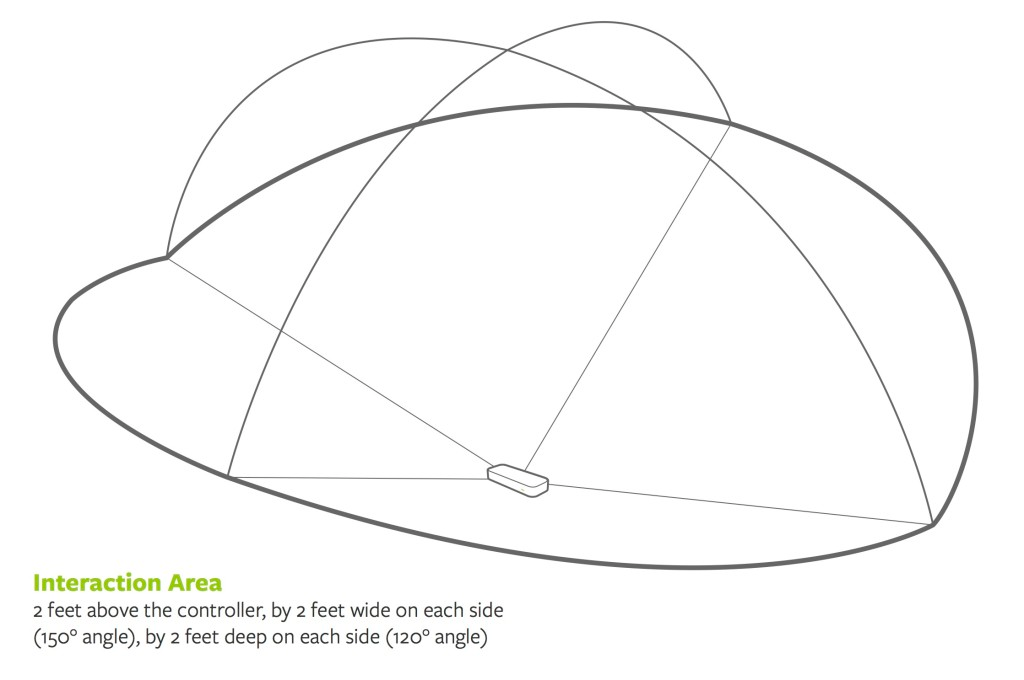
\includegraphics[ width = 14cm]{interactionArea}
\caption{Interaction area of Leap Motion device. \cite{area}}\label{area}
\end{figure}

Next will be displayed some advantages and disadvantages of Leap Motion controller that I think I have found.

\textbf{Advantages of Leap Motion controller}
\begin{itemize}
\item \textbf{Inexpensive.} As for other tracking devise out there Leap Motion costs arround 80 \$ without shippment and texes;
\item \textbf{Extremly precise motion control}.It can track the movement of both hands and all 10 fingers with up to 1/100th millimeter accuracy \cite{accuracy} and no visible latency;
\item \textbf{Easy to set up}. To make it work, Leap Motion only needs the software to be installed on the machine and to be properlly plugged in an USB port;
\item \textbf{It works with Windows and Mac and any size display};
\item \textbf{It is the most accurate sensor that is current available on the market};
\item \textbf{It's size is very small}.
\end{itemize}

Now let's see what are the disadvantages of Leap Motion.\\
\textbf{Disadvantages of Leap Motion controller}

\begin{itemize}
\item \textbf{Range of detection is limited}. After the last update of Leap Motion Orion, the range of detection got from 60 cm to 80 cm. However sometimes is not enough;
\item \textbf{Limited as a practical controller}. Is designed only to detect hands and finger tracking;
\item \textbf{Sensors does not always register hand position properly};
\item \textbf{Limited support}. There is still no support for other platforms such as Mobile, Linux;
\item \textbf{Facing upwards}. You have to put it facing upwards and interact in the abover region which might get a little awkward. People this days prefer sensors to be placed in front e.q. in the place of a webcam.
\end{itemize}
\textbf{Why I did choose to use Leap Motion over Microsoft Kinekt?}

Eventhough I have a Microsoft Kinekt also, I choosed to use Leap Motion because is a total new devise which may bring new possibilities of solving problems. It is rather simple to use and install and the price is much much less than to a Microsoft Kinekt. The documentation on how to integrate it in Unity is more.
It is more accurate sensor than Kinekt and it's size is very small which is an advantage. 
I thought that users, patients, hospitals, rehabilitation centers will appriciate it's advantages over Microsoft Kinekt.

\subsubsection {C\# or JavaScript?}

First I will talk about JavaScript. In Unity JavaScript is not the same as writing it for browsers(which is why it is popularly nicknamed UnityScript in the Unity's community).
UnityScript has so many shortcuts that are just invitations to make mistakes, sometimes programmer will lose the time just tracking bugs or mistakes. One of the biggest, most awful thing is implicit variable declaration. Following example in  \autoref{variable{} will explain it 

\begin{lstlisting}[caption={Implicit variable declaration in UnityScript.},label={variable}]

var myCounter;

void Update () 
    {
	 if (mycounter > 0)
	    {
	        // bla bla bla...
	    }
    }
\end{lstlisting}

Can you spot the error in there?. The variable of misspelled from myCounter to mycounter in Update, the compiler will create a new variable with a default value to 0, so the if will never happen, despite of what value myCounter get's in the editor.

There won't be warnings from the compiler, since implicit declaration is legal. This first reason is a must use C\# case.

The number 2 reasons is Visual Studio. As from 2016 Visual Studio now support Unity . With Intellisense and inline help, the API of Unity will be more easy to learn as you type. There is simply no better editor and debugger on the market, at least for .Net development.


And lastly, with C\# the developer has access to .Net meachanisms that have not been ported to UnityScript, which is Mono as a script host. While one can argue about merits of C\# as a language, Mono's base class library offers a wealth of functions. Collections, I/O, multithreading, and insanely expressive LINQ all speed up development considerably.

%----------------------------------------------------------------------------
\addtocontents{toc}{\protect\newpage}


\subsubsection {Leap Motion SDK}
\subsubsection{LitJSON}
JSON is a simple, yet powerful notation to specify data. It defines simple scalar types such as boolean, number (integers and reals) and string, and a couple of data structures: arrays (lists) and objects (dictionaries). For more information on the JSON format, visit JSON.org.

LitJSON is written in C\#, and it’s intended to be small, fast and easy to use. It was developed on a GNU/Linux environment, using the Mono framework.

In order to consume data in JSON format inside .Net programs, the natural approach that comes to mind is to use JSON text to populate a new instance of a particular class; either a custom one, built to match the structure of the input JSON text, or a more general one which acts as a dictionary.

Conversely, in order to build new JSON strings from data stored in objects, a simple export operation sounds like a good idea.

For this purpose, LitJSON includes the JsonMapper class, which provides two main methods used to do JSON-to-object   and object-to-JSON conversions. These methods are JsonMapper.ToObject  \autoref{litjson} and JsonMapper.ToJson.
\begin{lstlisting}[caption={LitJson usage example in C\# \cite{lit}.},label={litjson}]
using LitJson;
using System;

public class JsonSample
{
    public static void Main()
    {
        string json = @"
          {
            ""album"" : {
              ""name""   : ""The Dark Side of the Moon"",
              ""artist"" : ""Pink Floyd"",
              ""year""   : 1973,
              ""tracks"" : [
                ""Speak To Me"",
                ""Breathe"",
                ""On The Run""
              ]
            }
          }
        ";

        LoadAlbumData(json);
    }

    public static void LoadAlbumData(string json_text)
    {
        Console.WriteLine("Reading data from the following JSON string: {0}",
                          json_text);

        JsonData data = JsonMapper.ToObject(json_text);

        // Dictionaries are accessed like a hash-table
        Console.WriteLine("Album's name: {0}", data["album"]["name"]);

        // Scalar elements stored in a JsonData instance can be cast to
        // their natural types
        string artist = (string) data["album"]["artist"];
        int    year   = (int) data["album"]["year"];

        Console.WriteLine("Recorded by {0} in {1}", artist, year);

        // Arrays are accessed like regular lists as well
        Console.WriteLine("First track: {0}", data["album"]["tracks"][0]);
    }
}
\end{lstlisting}

In order to use LitJSON is needed to download the .dll file from their github page, add it to your project and then include the following code in every C\# script file, as shown in  \autoref{usingLitJson}
\begin{lstlisting}[caption={Using LitJSON as a json reader for your project.},label={usingLitJson}]
using LitJson;
\end{lstlisting}


For Kyno I used only JsonMapper.ToObject which helped me to easily read text from a text file. See for how it was implemented in subsection \textbf{Implementation}.

\subsubsection{APIs}
For the purpose of getting tracked data from the Leap Motion it is of a great use to use the API, which is a set of tools, routes, protocols used in order to build an applicaiton.

An API offers SaaS. This is a great benefit and opportunity for the programmers because they do not have to start programming from scratch every time they need to create a new software. APIs are very useful and they will be used in Kyno in order to get frame, hand, fingers tracking data from leapmotion and reading text from a file without having the programmers to write code from scratch, but focusing their attention on code that does what the APIs or framework can not do. 

An API is basically a method of software to speak with another software. So everytime the programmer wants to access a set of data he has to call the API. But the amount of data that can be accessed by him is limited so he has to communicate to the API in a very specific language.

In \mbox{figure \ref{api}} is visualized the concept of API as an middleman between a programmer and application. The one that accepts request and informs programmers about everything is middleman. However if the requested is allowed the middleman returns the data.
\begin{figure}[!h]
\centering
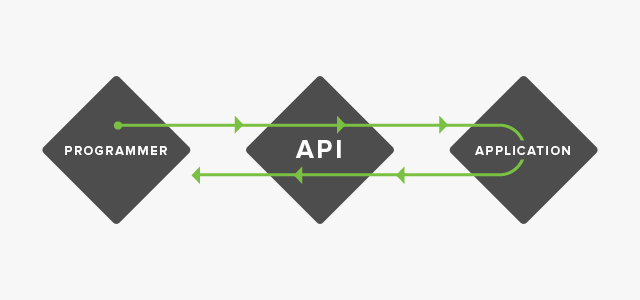
\includegraphics[ width = 10cm]{api}
\caption{Communication between programmer and application through API. \cite{api}}\label{api}
\end{figure}

For the implementation of having tracked data and then using it there are used the API of Leap Motion device.

\subsubsection{Leap Motion API}
At the very bottom level, the leap motion API returns the tracking data in the form of frames. Each Frame object contains lists of tracked entities, such as hands, fingers and tools, as well as objects representing recognized gestures and factors describing the overall motion of hands in the scene.

Motions are continuous hand movements – estimates of how the position of tracked objects (hands, fingers, and tools) change over time. These consist of translation, rotation, and scale. Comparing any two frames containing the same hand allows you to compute the change in motion through time.

The API is able to provide a wide range of additional tracking data, including left vs. right hands, tracking confidence values, as well as grab and pinch strength. Finger tracking is now persistent (so that each hand always has five fingers), digit types are identified (thumb, index, middle, ring, and pinky), and individual bones and joints are tracked.

In \mbox{figure \ref{leapapi}} is shown how the tracked entity in the Leap Motion is placed withing a hierarchy that starts with the hand. 

\begin{figure}[!h]
\centering
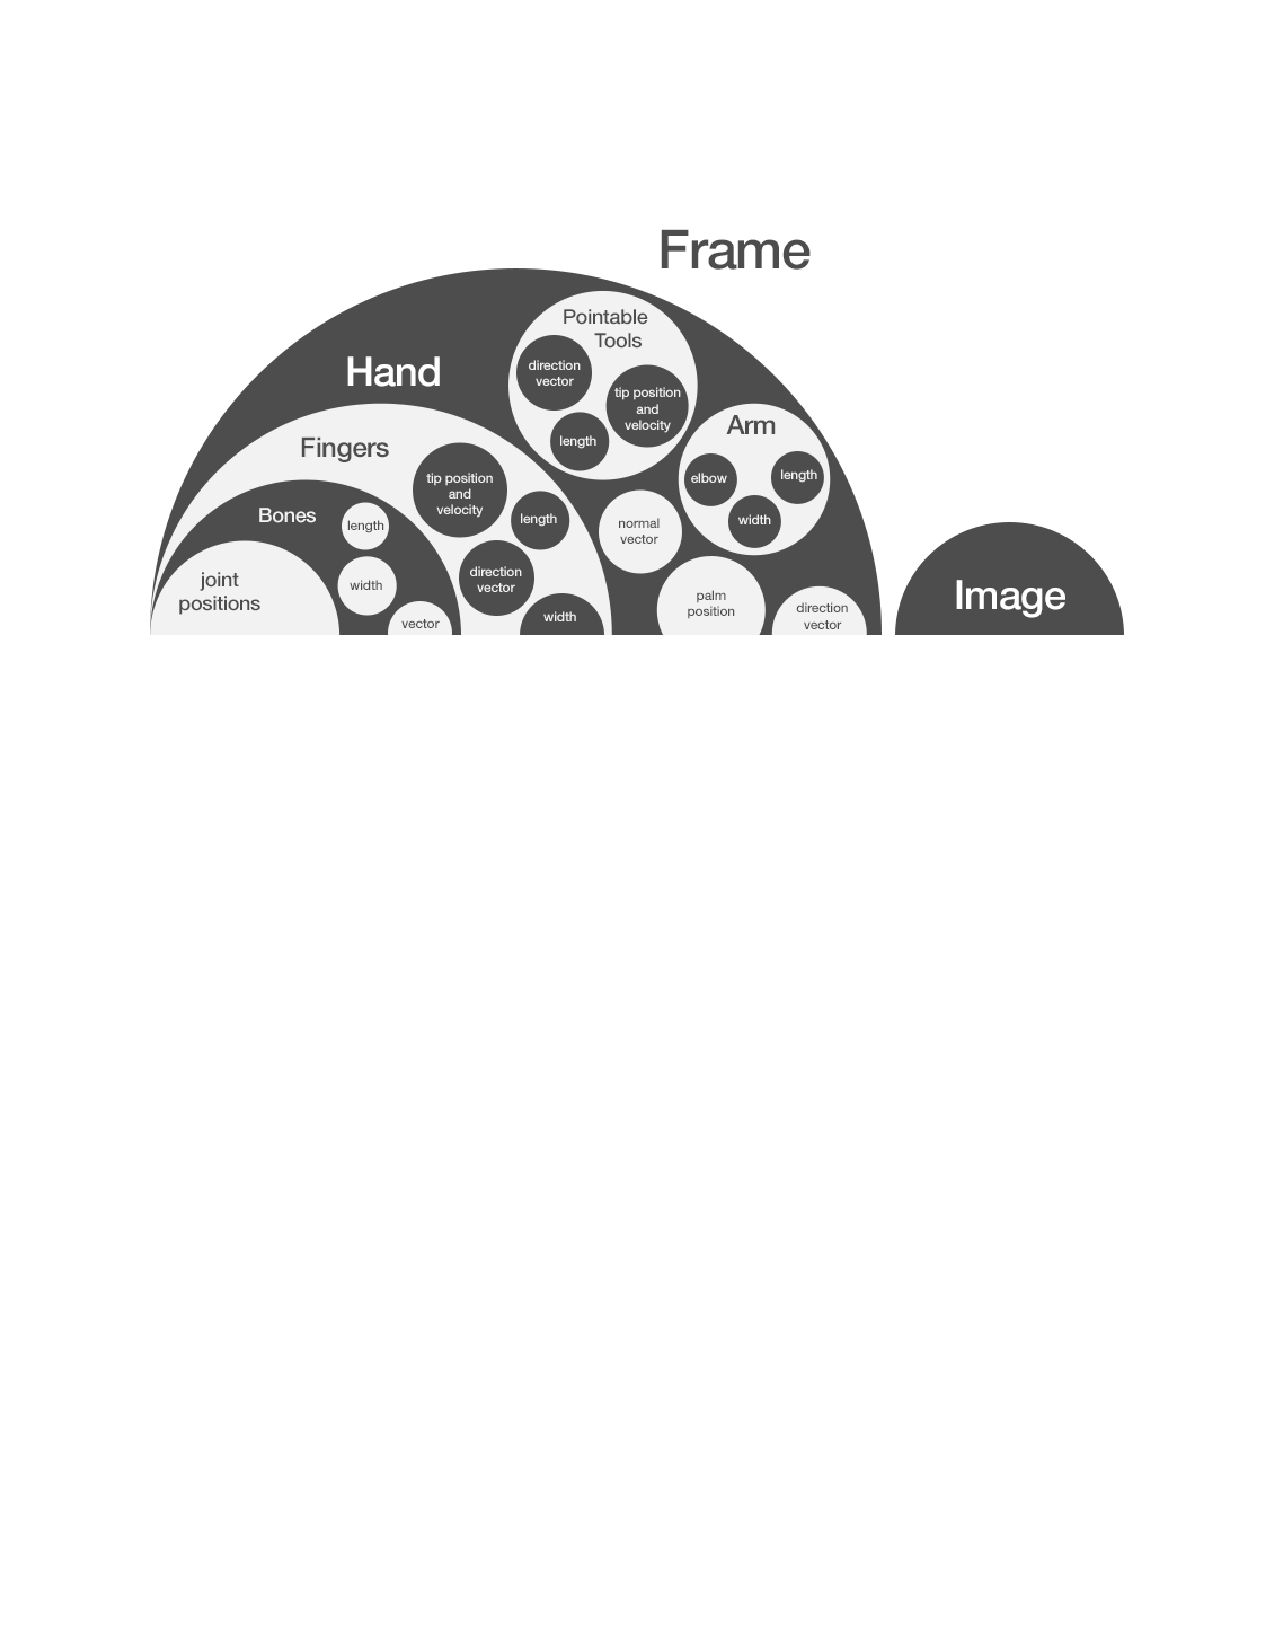
\includegraphics[trim={0 17cm 0 3cm},clip, width = 16cm]{leapapi}
\caption{Communication between programmer and application through API. \cite{leapapi}}\label{leapapi}
\end{figure}

A hand object includes: 
\begin{itemize}
\item palm position and velocity;
\item direction and normal vectors;
\item orthonormal basis.
\item \textbf{Fingers}. 
\begin{enumerate}
\item tip position and velocity;
\item direction vector;
\item orhonormal basis;
\item length and width.
\end{enumerate}
\item \textbf{Pointable Tools}
\begin{enumerate}
\item tip position and velocity;
\item direction vector;
\item length and width.
\end{enumerate}
\end{itemize}

And other components that are shown in \mbox{figure \ref{hand}}.
\begin{figure}[!h]
\centering
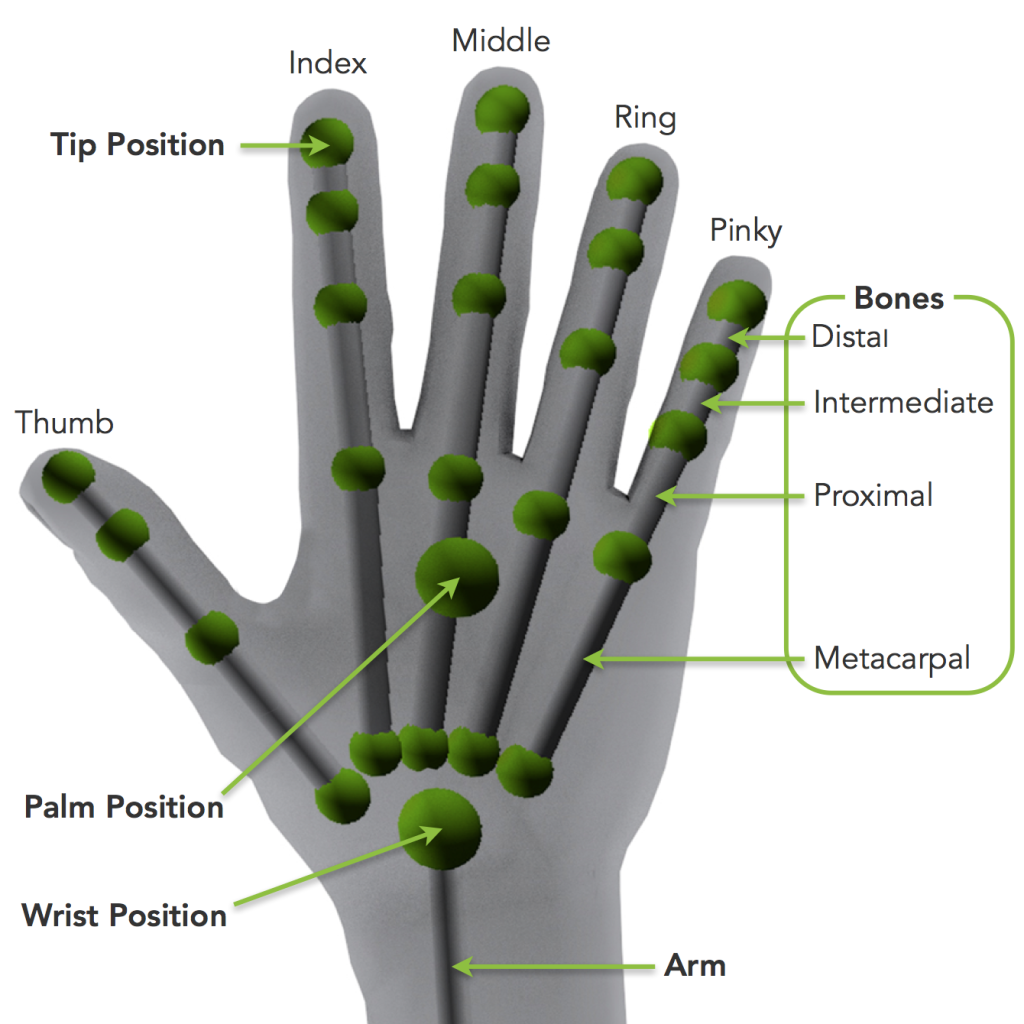
\includegraphics[ width = 14cm]{hand}
\caption{Components of Hand object in Leap Motion. \cite{leapapi}}\label{hand}

\end{figure}

In order to understand how it works this API we need to check the main components it provides to us:

\begin{itemize}
\item \textbf{Connecting to the controller}. Connecting to the Leap Motion controller.


To connect to the Leap Motion device, is needed to be created a Controller object 
\autoref{controller} . The Controller object establishes a connection automatically to the Leap Motion daemon which then passes tracking data in the form of Frame object to the application.

\begin{lstlisting}[caption={Controller object creation in C\#},label={controller}]
Controller controller = new Controller ();
\end{lstlisting}

Using controller object can be used to get information about the state of the connection and connected hardware and to set connection options to the application.


\item \textbf{Frames}. Getting tracking data from the API.

The Leap Motion API presents motion tracking data as a series of snapshots called frames. Each frame of tracking data contains the measured positions and other information about each entity detected in the snapshot.

Each Frame object contains snapshot of the scene recorded by the Leap Motion controller. Hands, fingers are the basic physical entities tracked.

A Frame contains tracked data from a connected Controller  \autoref{frames}object.

\begin{lstlisting}[caption={Accesing last and previous frame from a controller object.},label={frames}]
if (controller.IsConnected) { //controller is a Controller object
    Frame lastFrame = controller.Frame (); 
    Frame previousFrame = controller.Frame (1);
}
\end{lstlisting}

Then getting data from a frame as the basic objects tracked by the Leap Motion system is shown in \autoref{data}:

\begin{lstlisting}[caption={Getting data from a frame},label={data}]

Frame frame = controller.Frame ();
List<Hand> hands = frame.Hands;
\end{lstlisting}


The returned object by the Frame object are all read-only. They can be stored and used later in the future.

\item \textbf{Hands}. Tracking Hands.
Hands are the main entity tracked by the Leap Motion controller. The controller maintains an inner model of the human hand and validates the data from its sensors against this model. This allows the controller to track finger positions even when a finger is not completely visible. Note that it is possible for movement or changes in position to be lost when a finger is behind or directly in front of the hand (from the point of view of the controller). The Leap Motion software matches the internal model against the existing data. In some cases, the software can make an incorrect match – for example, identifying a right hand as a left hand.

The Hand class represents a physical hand detected by the Leap. A Hand object provides access to lists of its pointables as well as attributes describing the hand position, orientation, and movement.

Get Hand objects from a Frame:
\begin{lstlisting}[caption={Getting Hand from a Frame},label={hand}]
Frame frame = controller.Frame (); 
if(frame.Hands.Count > 0){
    List<Hand> hands = frame.Hands;
    Hand firstHand = hands [0];
}
\end{lstlisting}


\item \textbf{Fingers}. Tracking Fingers.
Fingers are represented by Pointable objects. In addition, a separate Finger class specializes the Pointable class to provide specific finger information.
The fingers can be get as a list or using an ID obtained in the previous frame. The next example is shown how to get the fingers by list:
\begin{lstlisting}[caption={Getting fingers from a Hand by list},label={fingers}]
List<Finger> fingers = hand.Fingers;
\end{lstlisting}
\item \textbf{Coordinate Systems}. Converting from Leap Motion to application coordinates.
A fundamental task when using the Leap Motion controller in an application is mapping the coordinate values received from the controller to the appropriate application-defined coordinate system.

The Leap Motion Controller provides coordinates in units of real world millimeters within the Leap Motion frame of reference. That is, if a finger tip’s position is given as (x, y, z) = [100, 100, -100], those numbers are millimeters – or, x = +10cm, y = 10cm, z = -10cm.

The Leap Controller hardware itself is the center of this frame of reference. The origin is located at the top, center of the hardware. That is if you touch the middle of the Leap Motion controller (and were able to get data) the coordinates of your finger tip would be [0, 0, 0].


In its normal position, that is on a desk with the user on one side and the computer monitor on the other, the user is “in front” (+z) of the controller and the monitor screen is “behind”(-z) the controller \mbox{figure \ref{coordinate}}. 

 
\begin{figure}[!h]
\centering
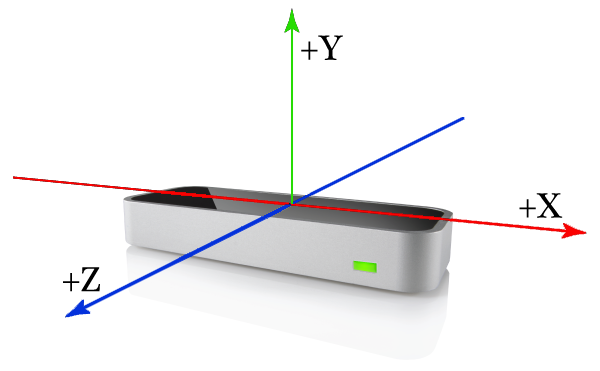
\includegraphics[ width = 10cm]{coordinate}
\caption{The Leap Motion controller uses a right-handed coordinate system. \cite{coordinates}}\label{coordinate}
\end{figure}


The Unity environment uses the left-hand rule, meaning the z axis points away from the user when the x axis is to the right and y is up. So, it needs to multiply Leap Motion coordinates by -1 \autoref{lefthand} for z axis to be map correctly in Unity3D.

\begin{lstlisting}[caption={Mapping right hand to left hand rule.},label={lefthand}]
Leap.Vector leapToWorld(Leap.Vector leapPoint, InteractionBox iBox)
{
    leapPoint.z *= -1.0f; //right-hand to left-hand rule
    Leap.Vector normalized = iBox.NormalizePoint(leapPoint, false);
    normalized += new Leap.Vector(0.5f, 0f, 0.5f); //recenter origin
    return normalized * 100.0f; //scale
}

\end{lstlisting}
\end{itemize}


\subsection{Implementation}
%developer.leapmotion.com/documentation/csharp/devguide/Leap_Hand.html


\subsubsection{Software license}
Kyno will be offered for a period of 1 month for free. In this period, the software will be tested and feedback will be prompted from users. It is very important at this stage to see how the application is doing, where are the problems, what features need to be added. 

After 1 month of free using, a monthly or yearly subscription plan will be applied with different prices for individual patients or hospitals and rehabilitation centers.


\subsubsection{BackEnd}

In order for the Leap Motion to work with the application it needs to be created a controller object \autoref{controller}. The Controller object establishes a connection automatically to the Leap Motion daemon which then passes tracking data in the form of Frame object to the application \autoref{matrix}.

\begin{lstlisting}[caption={Controller connection and frame setting},label={conroller}]
 protected virtual void Start() {
       createController();
       _untransformedUpdateFrame = new Frame();
     }
         protected void createController() {
           if (leap_controller_ != null) {
             destroyController();
           }
           leap_controller_ = new Controller();
         }
             protected void destroyController() {
               if (leap_controller_ != null) {
                 if (leap_controller_.IsConnected) {
                   leap_controller_.ClearPolicy(Controller.PolicyFlag.POLICY_OPTIMIZE_HMD);
                 }
                 leap_controller_.StopConnection();
                 leap_controller_ = null;
               }
             }
\end{lstlisting}



Now in the following listing it is extracted a transform matrix containing translation, rotation, and scale from a Unity Transform object and returns a Leap Motion LeapTransform object.
Using this matrix to transform Leap Motion tracking data to the Unity world relative to the
specified transform.

In addition to applying the translation, rotation, and scale from the Transform object, the returned
 transformation changes the coordinate system from right- to left-handed and converts units from millimeters to meters
by scaling.
It returns A Leap.LeapTransform object representing the specified transform from Leap Motion into Unity space.
\begin{lstlisting}[caption={Leap Motion tracking matrix data.},label={matrix}]
protected void updateIfTransformMoved(Frame source, ref Frame toUpdate) {
      if (transform.hasChanged) {
        _transformedUpdateFrame = null;
        transform.hasChanged = false;
      }

      if (toUpdate == null) {
        toUpdate = source.TransformedCopy(transform.GetLeapMatrix());
      }
    } 
\end{lstlisting}

Next in \autoref{update} is how to update the graphical part of hand representation by taking the current frame each time the update function is executed. And then passing it to a hand factory which contains the current hands displayed on the screen and from there it will set the updating data each time a frame is generated.

\begin{lstlisting}[caption={Updating hand representations },label={update}]
  protected LeapProvider provider;
  protected HandFactory factory;
  
    protected virtual void Start() {
        provider = requireComponent<LeapProvider>();
        factory = requireComponent<HandFactory>();
      }
      
       protected virtual void Update() {
            Frame frame = provider.CurrentFrame;
      
            if (frame != null && graphicsEnabled) {
              UpdateHandRepresentations(graphicsReps, ModelType.Graphics, frame);
            }
          }
\end{lstlisting}

From here  using the factory object, each hand's data such as position, scale, rotation of the hand can be get and mapped to a virtual hand in Unity. 

A lot of back magic was made by Leap Motion they provided a package for Unity where there are scripts and prefabs ready to be used in development and these prefabs will provide the developer with a set of virtual hand. As for me as a developer, I was able to focus more on the practical part of the application by implementing the gestures I planned to have in the application.

\textbf{Pinch}

Leap Motion's API provide pinching only with the index finger. In order to get a pinch with other finger it need to be calculated the distance between Thumb and rest of the fingers. For that in \autoref{pinch} at line 19 is provided a functiont that will return the distance between 2 fingers or better say tip position of the fingers. So every time GetDistanceToThumb will be called it will calculate that distance. By default the API returns the distance in mm so I had somehow to convert it to a better form for the purpose of later usage in the code.

\begin{lstlisting}[caption= {Pinching detection in Kyno},label={pinch}]

 protected void FingerTips(Hand h)
    {
      Dictionary<string, Vector3> fingerInfo = new Dictionary<string, Vector3>();
      List<Finger> fingers = h.Fingers;

      foreach (Finger finger in fingers)
      {
        fingerInfo.Add(finger.Type.ToString(), finger.TipPosition.ToVector3());
      }


      var toIndexDist = GetDistanceToThumb(fingerInfo, 0, 1);
      var toMiddleDist = GetDistanceToThumb(fingerInfo, 0, 2);
      var toRingDist = GetDistanceToThumb(fingerInfo, 0, 3);
      var toPinkyDist = GetDistanceToThumb(fingerInfo, 0, 4);
      
}
 protected float GetDistanceToThumb(Dictionary<string, Vector3> fingers, int firstPosition, int secondPosition)
    {
      float distance = (float)Math.Round(Vector3.Distance(fingers.ElementAt(firstPosition).Value, fingers.ElementAt(secondPosition).Value), 4) * 10.0f;
      return distance;
    }
\end{lstlisting}

After getting the distance from Thumb to other tip of the fingers I could check if there would be a pinch or not.

\textbf{Grab}

%developer..leapmotion.com/documentation/java/api/Leap.Pointable.html#javaclasscom_1_1leapmotion_1_1leap_1_1_pointable_1ada0cf872bb60b0b7b8d2ab94f4c77047
A finger is considered extended if it is extended straight from the hand as if pointing. A finger is not extended when it is bent down and curled towards the palm.

So here I just had to check if all of the fingers are not extended and if not that it will be a grab otherwise it won't be.
\begin{lstlisting}[caption={Grab detection in Kyno},label={createController}]
 void Update()
    {
      if (canGrab)
      {
        Debug.Log("Can Grab");
        ensureGrabInfo();
      }
    }
  protected virtual void ensureGrabInfo()
    {
      Hand hand = _handModel.GetLeapHand();
      var fingers = hand.Fingers;
      grabDetection(fingers);
    }
    
     protected virtual void grabDetection(List<Finger> fingers)
        {
          if (!fingers.Any(o => o.IsExtended))
          {
            //StartCoroutine(DoTheDance());
            if(canGrow)
              SetCounter();
            Debug.Log("Its a full finger grab!!!");
          }
          else
          {
            Debug.Log("Its not a full finger grab");
            canGrow = true;
          }
        }
\end{lstlisting}


\textbf{Rotate}

Rotation is quite tricky but not possible to detect tanks to Leap Motion. Using normal vector to the palm.

If your hand is flat, this vector will point downward, or “out” of the front surface of your palm.

The direction is expressed as a unit vector pointing in the same direction as the palm normal (that is, a vector orthogonal to the palm).

It can be used the palms normal vector to compute the roll angle of the palm with respect to the horizontal plane as it shown in line 12 of the following  code snippet: 
\begin{lstlisting}[caption={Rotation detection in Kyno},label={createController}]
void Update()
    {
      if (canRoll)
      {
        ensureRollInfo();
      }
    }

    protected virtual void ensureRollInfo()
    {
      Hand hand = _handModel.GetLeapHand();
      float roll = -hand.PalmNormal.Roll;
      float rollDegrees = ToDegrees(roll);
      Debug.Log(rollDegrees);
      if((rollDegrees > 85 || rollDegrees < -85))
      {
        if(canGrow)
          SetCounter();
      }

      else
      {
        canGrow = true;
      }
    }

    protected float ToDegrees(float Radian)
    {
      float Degrees;
      Degrees = Radian * 180 / Mathf.PI;
      return Degrees;
    }
\end{lstlisting}
 
 The angle on which the hand was rotated will be returned in radians so in order to transform it in angle ToDegree method was implemented. 
 
 Rotate, grab and pinch is executed in Update function which means that it will be called once per frame.
 
 \subsubsection{UI of Kyno application}
  In this section is described how the UI in Kyno was implemented, from the pie menu that is at the bottom left corner of the screen to the tips pannel on the right side of the screen. In \autoref{readJsonCode} is shown how the text file is loaded from an json file and saved to an object of JsonData type. Than by with the help of readJson variable the data that was saved in the itemData variable will be accessed from another script. Also Awake function is called at the moment when the application is started so the reading will be made at this stage.
  
  
 \begin{lstlisting}[caption={Reading JSON from a file.},label={readJsonCode}]
 using LitJson;

   private string jsonString;
   public JsonData itemData;
   public static ReadJson readjson;
   void Awake()
   {
     TextAsset text = Resources.Load("Items") as TextAsset;
     jsonString = text.text;
      itemData = JsonMapper.ToObject(jsonString);
   }
   public JsonData GetItem(string value, string type) 
   {
     for (int i = 0; i < itemData[type].Count; i++)
     {
       if (itemData[type][i]["value"].ToString() == value)
         return itemData[type][i];
     }
     return null;
   }
 \end{lstlisting}
 
 
One way to not overpopulate the screen with different graphics that will give distraction to the user is to close the panels/menu as much as possible. One solution is shown in \autoref{Tips} where the panel with the tips for user is displayed/hidden at a button press.
 \begin{lstlisting}[caption={Moving tips panel},label={Tips}]
   void Start()
 	{
 		oldPosition = transform.position;
 	}
 	
 	// Update is called once per frame
 	void Update ()                                                 
 	{
     if (moved)
       PositionChanging(step);
    else
       PositionChanging(0);
   }
   //position change in relation to the new distance
   public void PositionChanging(float distance)
   {
     if (!firstMove) { 
       Vector3 newPosition = new Vector3(oldPosition.x + distance, oldPosition.y,
                                          oldPosition.z);
       transform.position = Vector3.Lerp(transform.position, newPosition, Time.deltaTime * smooth);
     }
   }
   //toggle the moved boolean
   public void Open()
 	{
 		moved = true;
 	}
 
   public void Close()
   {
     moved = false;
   }
 \end{lstlisting}

 Next is described in the \autoref{pie} is described how the menu is placed in a circular way. For a better vizualizing experience at the application launch the user is prompt with a welcome screen. During that time Move function must wait some seconds in order to start, for this is used coroutines which will delay the running of Wait with required time.
  
    \begin{lstlisting}[caption={Coroutines},label={pie}]
      private IEnumerator Wait(float smoothScale, float smoothingPos, float angle)
      {
        yield return new WaitForSeconds(intro.waitingTime  + 2);
        StartCoroutine(Move(smoothingScale, smoothingPos, angle));
      }
    \end{lstlisting}
 Coroutines are computer program components that generalize subroutines for nonpreemptive multitasking, by allowing multiple entry points for suspending and resuming execution at certain locations. Coroutines are well-suited for implementing more familiar program components such as cooperative tasks, exceptions, event loop, iterators, infinite lists and pipes. 
 
 In \autoref{pie} is described the itself action on generating a pie menu. First of all in order to place some graphics in a circular path we need to find the points of that circular path. For this the parapetric equation of a circle come in hand. 
 A circle can be defined as the locus of all points that satisfy the equations
 $x = r cos(t)$ and    $y = r sin(t)$
 
 where x,y are the coordinates of any point on the circle, r is the radius of the circle and 
 t is the parameter - the angle subtended by the point at the circle's center. Hence the pie menu will be displayed only on $1/4$ of a full circle the angle will be only $\pi/2$
  \begin{lstlisting}[caption={Creation of a Pie Menu},label={createController}]
   private IEnumerator Move(float smoothScale, float smoothingPos, float a)
    {
      while (true) {
        for (int i = 0; i < numPoints; i++)
        {
          //multiply 'i' by '1.0f' to ensure the result is a fraction
          float pointNum = (i * 1.0f) / numPoints;
          //angle along the unit circle for placing points
          float angle = pointNum * a;
  
          float x = Mathf.Sin(angle) * radiusX;
          float y = Mathf.Cos(angle) * radiusY;
  
          //position for the point prefab
          if (vertical)
            pointPos = new Vector3(x, y) + centerPos;
          else if (!vertical)
          {
            pointPos = new Vector3(x, 0, y) + centerPos;
          }
          //place the prefab at given position
          axis = pieButton[i].GetComponent<RectTransform>().localPosition - pointPos;
          axis.Normalize();
          pieButton[i].GetComponent<RectTransform>().localPosition = Vector3.Lerp(pieButton[i].GetComponent<RectTransform>().localPosition, pointPos * axis, smoothingPos * Time.deltaTime);
          pieButton[i].GetComponent<RectTransform>().localScale = Vector3.Slerp(pieButton[i].GetComponent<RectTransform>().localScale, Vector3.one, smoothingScale * Time.deltaTime);
        }
        yield return null;
      }
    }
  \end{lstlisting}
Now the placing on the path is rather simple. In order to display evenly the graphics on line 9 it is calculated a new angle for each of the graphic where it will be placed. Then again for each graphic on line 11 and 12 it will be calculted 2 float variables with info of the position of the current graphic. On line 16 or 19 it will be created a new Vector3 with coordinates of the point on the circle calculated earlier. Where on the 24 line the current graphic component will take this new Vector and it will Lerp through current position and the new position. In result the following  \mbox{figure \ref{pieMenu}} is displayed to the user 

 

 
\begin{figure}[!h]
\centering

\includegraphics[ width = 5cm]{pieMenu}
\caption{Panel with tips for user. }\label{pieMenu}
\end{figure}




The next \autoref{setData} is recieving information about the action it was made in the application and then it spreads the required data to the right text and image game objects of the application. With the help of the j parameter that is of ReadJson at Awake time it get's the ReadJson script component. With this parameter it will be possible to be accessed the JSON object that was saved when the JSON file was readen.

By specifying in the Unity editor which button it was pressed through accesing the parameter on the pushedButton function it can then be easily set the corresponding data as it can be seen in SetInfo function.
\begin{lstlisting}[caption={Data popularization},label={setData}]

  private static ReadJson j;

	// Update is called once per frame
	void Update () {
    Message();
	}
  void Awake()
  {
    j = this.GetComponent<ReadJson>();
    textReference.text = "";
  }
  private void SetInfo()
  {
    switch (pressedButton)
    {
      case "Grab":
        selectedText = j.GetItem(pressedButton, "tips")["text"].ToString();
        leftImageName = j.GetItem(pressedButton, "tips")["img1"].ToString();
        rightImageName = j.GetItem(pressedButton, "tips")["img2"].ToString();
        break;

      case "Roll":
        selectedText = j.GetItem(pressedButton, "tips")["text"].ToString();
        leftImageName = j.GetItem(pressedButton, "tips")["img1"].ToString();
        rightImageName = j.GetItem(pressedButton, "tips")["img2"].ToString();
        break;
      case "Pinch":
        selectedText = j.GetItem(pressedButton, "tips")["text"].ToString();
        leftImageName = j.GetItem(pressedButton, "tips")["img1"].ToString();
        rightImageName = j.GetItem(pressedButton, "tips")["img2"].ToString();
        break;
      default:
        Debug.Log("Default case");
        break;
    }

    ChangeInfo(selectedText, leftImageName, rightImageName);
  }
  private void ChangeInfo(string s, string image1, string image2)
  {
    textReference.text = s;
    leftImage.sprite = Resources.Load<Sprite>("Images/" + image1);
    rightImage.sprite = Resources.Load<Sprite>("Images/" + image2);

  }
  public void PushedButton(string s)
  {
    pressedButton = s;
    SetInfo();
  }
\end{lstlisting}

\mbox{Figure \ref{rightMenu}} is after data popularization when the user pressed the pinch button. This panel will provide user with some tips and images on how to do an exercise.

\begin{figure}[!h]
\centering

\includegraphics[width = 5cm]{rightMenu}
\caption{In application pie menu. }\label{rightMenu}
\end{figure}


\clearpage